%Correct the file name.
%X: book number
%Y: part number
%ZZZ: page number in three digits. So page 3 would be 003.

\documentclass[11pt]{amsbook}

\usepackage{../HBSuerDemir}	% ------------------------


\begin{document}

% ++++++++++++++++++++++++++++++++++++++
\hPage{b2p2/315}


\begin{hEnumerateAlpha}
	\item $f(1,1) = f(2,3)+(1-2)f_x (x^* + y^* ) + (1-3)f_y (x^* , y^* ) \\  \Rightarrow 4 = 59 - (8 {x^*}^3 + 3 {y^*}^2) - 2(6 x^* y^*	- 3 {y^*}^2) \\ \Rightarrow 55 = 8 {x^*}^3 + 12 x^* y^* \hfill(1)$
\end{hEnumerateAlpha}

\begin{center}
Since $(x^* , y^*)$ lies on $AB$ , we have 
$$ y^* = 2 x^* -1 \hfill(2) $$
and (1), (2) give
$$ \varphi (x^*) = 8 {x^*}^3 + 24 {x^*}^2 - 12 x^* -55 = 0 $$
\end{center}

\par Since $\varphi (1) = -35 < 0 $ , $\varphi (2) = 81 >0 $ hold , $x^*$ must lie between 1 and 2.

\begin{exmp}
Given 
$$ f(x,y)= \arctan \frac{y}{x}  $$
\begin{hEnumerateAlpha}
\item obtain TAYLOR's Formula with $R_3$ at $A(1,\sqrt{3})$
\item evaluate $f(2,3)$
\item Show existence of $(x^* , y^* )$ on the open line segment joining $A(1,\sqrt{3})$ to $B(\sqrt{3},1)$
\end{hEnumerateAlpha}
\begin{hSolution}
\begin{hEnumerateAlpha}
\item $f(x,y)=f(1,\sqrt{3}) + [(x-1)f_x (A) + (y-\sqrt{3}) f_y (B)] + \frac{1}{2}[(x-1)^2 f_{xx} (A) + 2 (x-1)(y-\sqrt{3}) f_{xy} (A) + (y-\sqrt{3})^2 f_{yy} (A) ] + R_3$
\newline where 

\par $f(1,\sqrt{3}) = \frac{\pi}{3} , f_x (A) = - \frac{\sqrt3}{4} , f_y (A) = \frac{1}{4} , f_{xx} (A) = \frac{\sqrt3}{8} , f_{xy} (A) = \frac{1}{8} , f_{yy} (A)= - \frac{\sqrt3}{8}$ \par $f(x,y)= \frac{\pi}{3} + [-\frac{\sqrt3}{4}(x-1) + \frac{1}{4}(y-\sqrt3)]
+ \frac{1}{2}[\frac{\sqrt3}{8} (x-1)^2 + \frac{1}{4} (x-1)(y-\sqrt3)-\frac{\sqrt3}{8} (y-\sqrt3)^2] + R_3$
\end{hEnumerateAlpha}
\end{hSolution}
\end{exmp}
% =======================================================
\end{document}  

%==== templates ====

%==== environments ====

%\begin{figure}[htb]
%	\centering
%	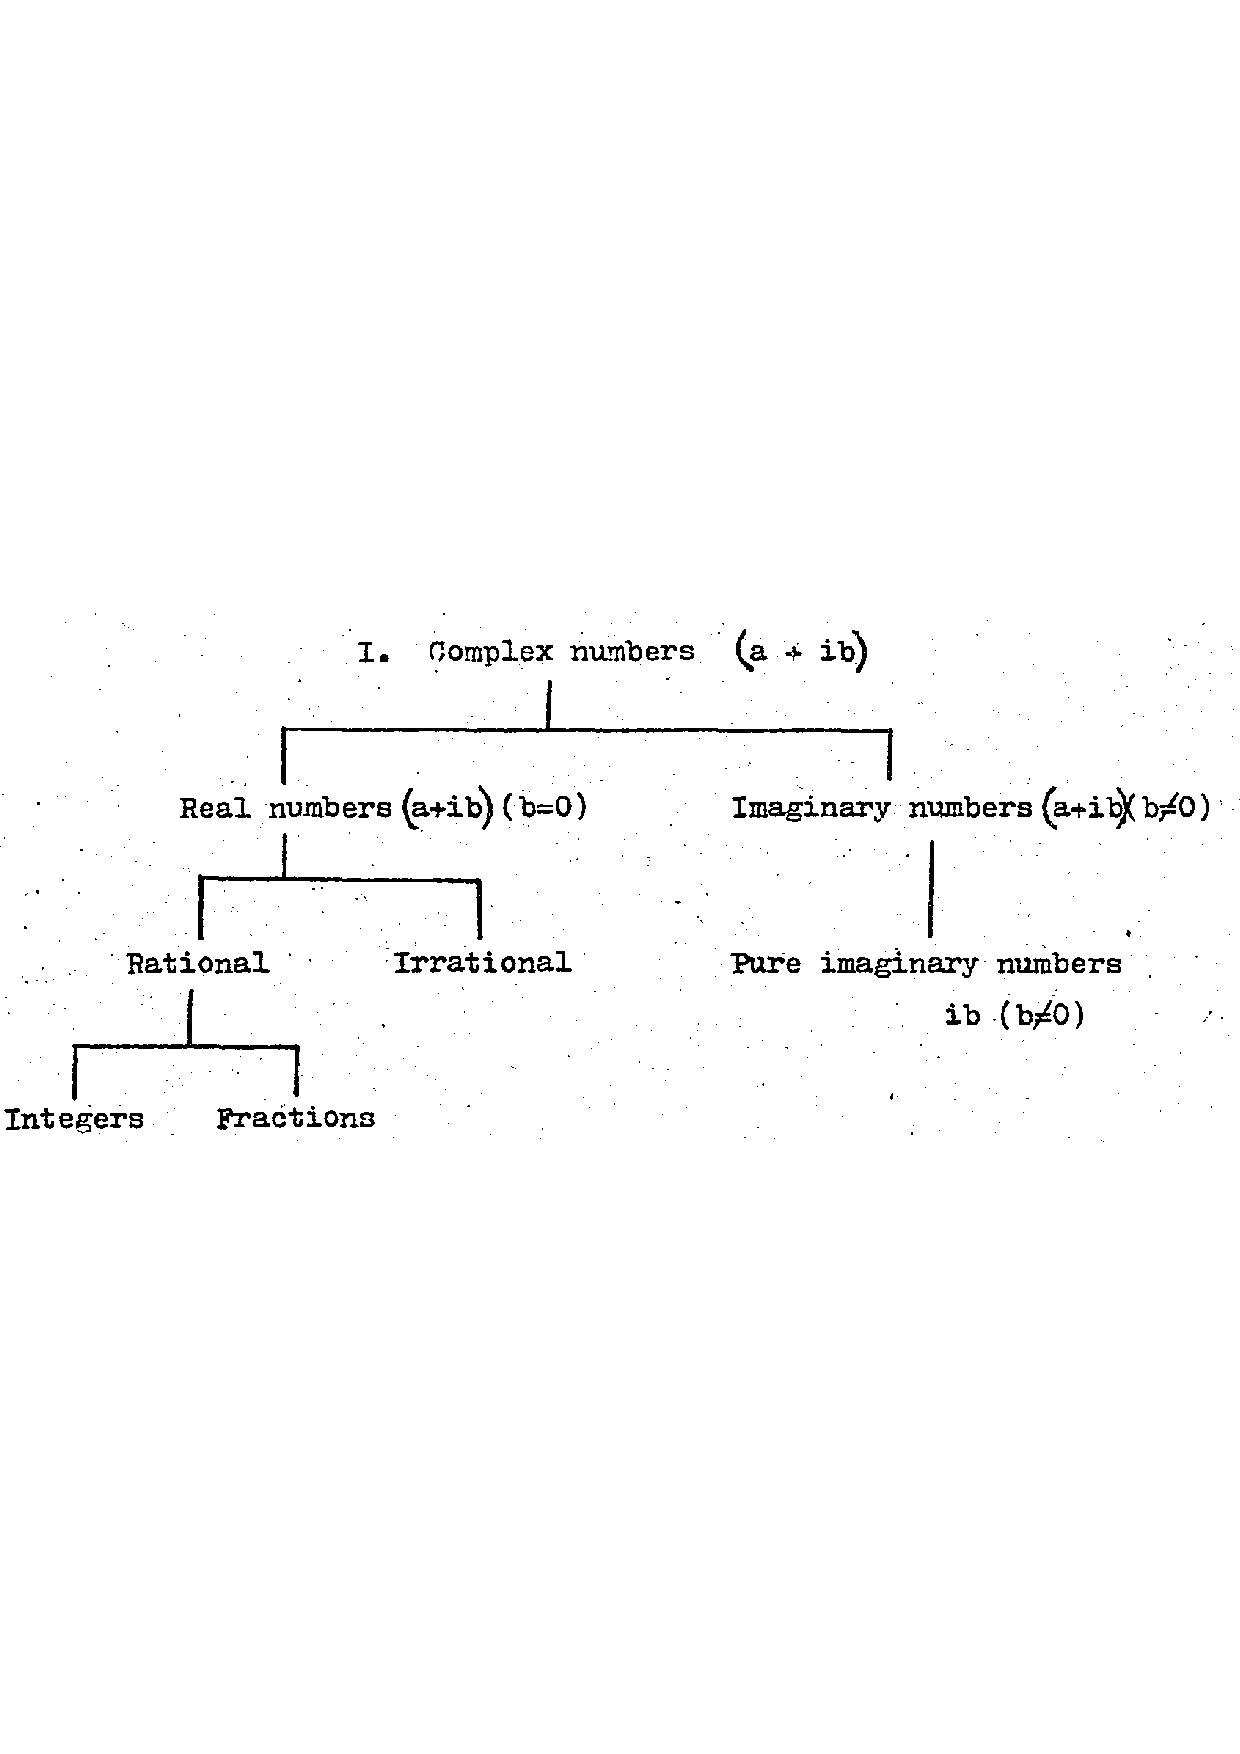
\includegraphics[width=0.9\textwidth]{images/SD-1-1p15A}
%	\caption{Classification of complex numbers}
%	\label{fig:classificationOfComplexNumbersA}
%\end{figure}

%\begin{center}
%\begin{tabular}{cc}
%\end{tabular}
%\end{center}

%\begin{exmp}
%\begin{hSolution}
%\end{hSolution}
%\end{exmp}

%\begin{hEnumerateAlpha}
%\end{hEnumerateAlpha}

%\begin{hEnumerateRoman}
%\end{hEnumerateRoman}

%$
%\begin{bmatrix}
%\end{bmatrix}
%$

%\frac{aaaa}{bbb}
%\frac{a_{n}}{b_{n}}
%\left( aaaa \right)
%\Longrightarrow

%\begin{multicols}{2}
%	bb
%\columnbreak
%	aa
%\end{multicols}
